% Standalone TikZ figure: PALL-Adapter Architecture
% Compile with: pdflatex architecture_tikz.tex
\documentclass[tikz,border=5pt]{standalone}
\usepackage{tikz}
\usetikzlibrary{arrows.meta, positioning, fit, backgrounds, calc, decorations.pathreplacing}
\usepackage{amsmath,amssymb}

\begin{document}
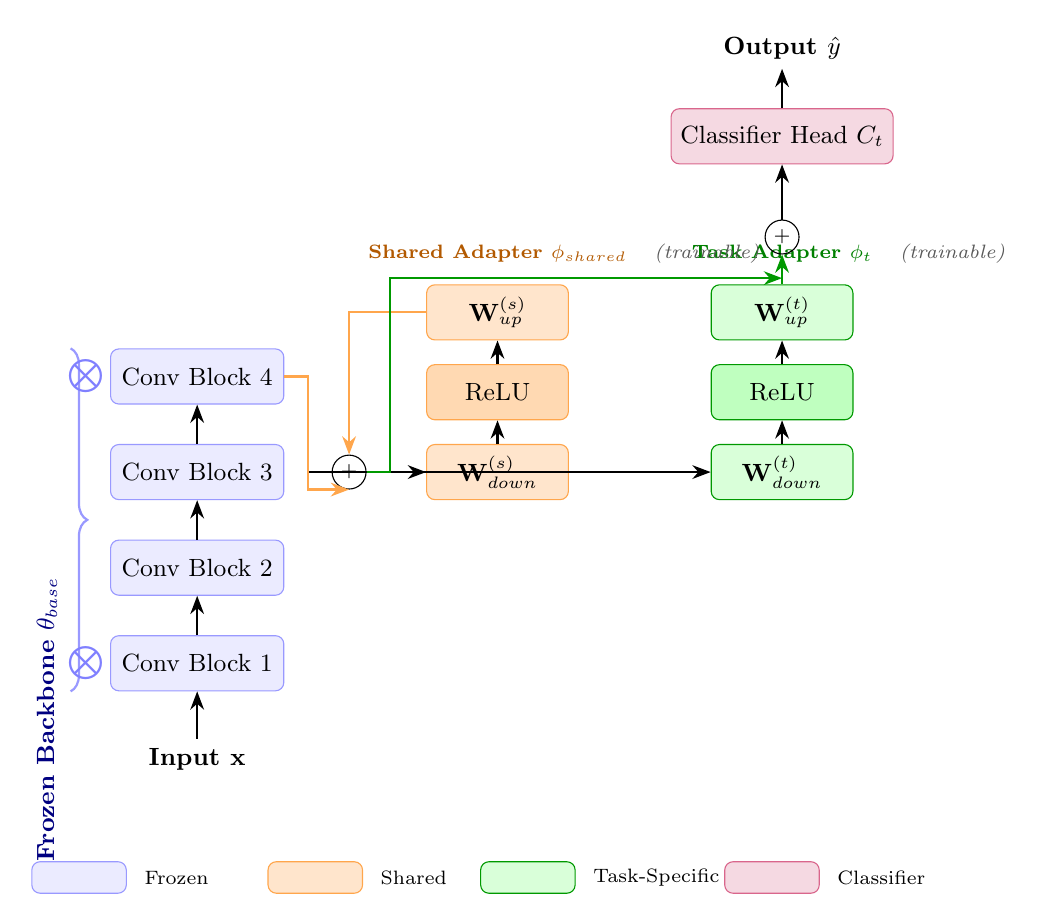
\begin{tikzpicture}[
    >=Stealth,
    node distance=0.8cm and 1.2cm,
    block/.style={rectangle, draw, rounded corners=3pt, minimum width=2.2cm, minimum height=0.7cm, align=center, font=\small},
    frozen/.style={block, fill=blue!8, draw=blue!40, text=black},
    shared/.style={block, fill=orange!20, draw=orange!70, text=black},
    task/.style={block, fill=green!15, draw=green!60!black, text=black},
    classifier/.style={block, fill=purple!15, draw=purple!60, text=black},
    arrow/.style={->, thick, >=Stealth},
    dasharrow/.style={->, thick, >=Stealth, dashed, gray},
    label/.style={font=\scriptsize\itshape, text=gray!70!black},
    phase/.style={font=\scriptsize\bfseries, text=red!70!black},
]

% === Input ===
\node (input) [font=\small\bfseries] {Input $\mathbf{x}$};

% === Frozen Backbone ===
\node (bb1) [frozen, above=0.6cm of input] {Conv Block 1};
\node (bb2) [frozen, above=0.5cm of bb1] {Conv Block 2};
\node (bb3) [frozen, above=0.5cm of bb2] {Conv Block 3};
\node (bb4) [frozen, above=0.5cm of bb3] {Conv Block 4};

% Backbone label
\node[rotate=90, font=\small\bfseries, text=blue!50!black, left=0.8cm of bb2] (bblabel) {Frozen Backbone $\theta_{base}$};
\draw[decorate, decoration={brace, amplitude=6pt, mirror}, blue!40, thick]
    ([xshift=-0.5cm]bb1.south west) -- ([xshift=-0.5cm]bb4.north west);

% === Shared Adapter (to the right of backbone) ===
\node (sa_down) [shared, right=1.8cm of bb3, minimum width=1.8cm] {$\mathbf{W}_{down}^{(s)}$};
\node (sa_relu) [shared, above=0.3cm of sa_down, minimum width=1.8cm, fill=orange!30] {ReLU};
\node (sa_up) [shared, above=0.3cm of sa_relu, minimum width=1.8cm] {$\mathbf{W}_{up}^{(s)}$};

% Shared adapter label
\node[font=\scriptsize\bfseries, text=orange!70!black, above=0.15cm of sa_up] (salabel) {Shared Adapter $\phi_{shared}$};

% === Task Adapters (to the right of shared) ===
\node (ta_down) [task, right=1.8cm of sa_down, minimum width=1.8cm] {$\mathbf{W}_{down}^{(t)}$};
\node (ta_relu) [task, above=0.3cm of ta_down, minimum width=1.8cm, fill=green!25] {ReLU};
\node (ta_up) [task, above=0.3cm of ta_relu, minimum width=1.8cm] {$\mathbf{W}_{up}^{(t)}$};

% Task adapter label
\node[font=\scriptsize\bfseries, text=green!50!black, above=0.15cm of ta_up] (talabel) {Task Adapter $\phi_{t}$};

% === Residual connections ===
\node (plus1) [draw, circle, inner sep=1.5pt, font=\scriptsize\bfseries, right=0.6cm of bb3] {$+$};
\node (plus2) [draw, circle, inner sep=1.5pt, font=\scriptsize\bfseries] at ($(ta_up.north)+(0,0.6)$) {$+$};

% === Classifier ===
\node (clf) [classifier, above=0.7cm of plus2, minimum width=2.2cm] {Classifier Head $C_t$};
\node (output) [font=\small\bfseries, above=0.5cm of clf] {Output $\hat{y}$};

% === Arrows: backbone flow ===
\draw[arrow] (input) -- (bb1);
\draw[arrow] (bb1) -- (bb2);
\draw[arrow] (bb2) -- (bb3);
\draw[arrow] (bb3) -- (bb4);

% Backbone to shared adapter
\draw[arrow] (bb4.east) -- ++(0.3,0) |- (sa_down.west);
\draw[arrow] (sa_down) -- (sa_relu);
\draw[arrow] (sa_relu) -- (sa_up);

% Residual: backbone output + shared adapter output
\draw[arrow, orange!70] (bb4.east) -- ++(0.3,0) |- (plus1.south);
\draw[arrow, orange!70] (sa_up.west) -| (plus1.north);

% Shared output to task adapter
\draw[arrow] (plus1.east) -- ++(0.3,0) |- (ta_down.west);
\draw[arrow] (ta_down) -- (ta_relu);
\draw[arrow] (ta_relu) -- (ta_up);

% Residual: shared output + task adapter output
\draw[arrow, green!60!black] (plus1.east) -- ++(0.3,0) |- ([yshift=-0.3cm]plus2.south);
\draw[arrow, green!60!black] (ta_up) -- (plus2);

% To classifier
\draw[arrow] (plus2) -- (clf);
\draw[arrow] (clf) -- (output);

% === Lock icons (frozen) ===
\node[font=\large, text=blue!50] at ([xshift=-0.3cm]bb1.west) {$\bigotimes$};
\node[font=\large, text=blue!50] at ([xshift=-0.3cm]bb4.west) {$\bigotimes$};

% === Trainable indicators ===
\node[label, right=0.1cm of salabel] {(trainable)};
\node[label, right=0.1cm of talabel] {(trainable)};

% === Legend ===
\begin{scope}[shift={(-1.5,-1.5)}]
    \node[frozen, minimum width=1.2cm, minimum height=0.4cm, font=\scriptsize] at (0,0) (leg1) {};
    \node[font=\scriptsize, right=0.1cm of leg1] {Frozen};
    \node[shared, minimum width=1.2cm, minimum height=0.4cm, font=\scriptsize] at (3,0) (leg2) {};
    \node[font=\scriptsize, right=0.1cm of leg2] {Shared};
    \node[task, minimum width=1.2cm, minimum height=0.4cm, font=\scriptsize] at (5.7,0) (leg3) {};
    \node[font=\scriptsize, right=0.1cm of leg3] {Task-Specific};
    \node[classifier, minimum width=1.2cm, minimum height=0.4cm, font=\scriptsize] at (8.8,0) (leg4) {};
    \node[font=\scriptsize, right=0.1cm of leg4] {Classifier};
\end{scope}

\end{tikzpicture}
\end{document}
